%\documentclass[14pt]{report}%{book}

\documentclass[LaM,binding=0.6cm]{sapthesis}
\usepackage{amsmath} % assumes amsmath package installed
\usepackage{amssymb}  % assumes amsmath package installed
\usepackage{graphicx}

\usepackage{microtype}
\usepackage{lipsum}
\usepackage{curve2e}
\usepackage{hyperref}
\usepackage{lettrine}
\usepackage{natbib}
%\usepackage{biblatex}
\usepackage{wrapfig}
\usepackage{color}
\usepackage{caption}
\usepackage{titlesec}
%\usepackage{subfigure}
\usepackage[raggedright]{sidecap}
\usepackage[table]{xcolor}
\usepackage{changepage}
\usepackage{tikz-cd}
\usepackage{algorithm}
%\usepackage{algorithmic}
\usepackage[noend]{algpseudocode}
%\usepackage{subcaption}
\usepackage{xcolor}

\usepackage[titletoc]{appendix}

% Consente di definire in modo flessible note e titoli
\usepackage{fancyhdr}
\pagestyle{fancy} 

\usepackage{calc}

\usepackage{makecell}
\usepackage{subfig}
\newcommand{\NE}{\mathbfsymbol{\rm{NE}}}
\newcommand{\sbt}{\,\begin{picture}(-1,1)(-1,-3)\circle*{3}\end{picture}\ }
\def\Real{\mathbb{R}}
\def\tm{\leavevmode\hbox{$\rm {}^{TM}$}}
\def\Complex{\mathbb{C}}
\usepackage{mathtools}
\newcommand\numberthis{\addtocounter{equation}{1}\tag{\theequation}}
\usepackage{array}
\newcolumntype{P}[1]{>{\centering\arraybackslash}p{#1}}
\newcolumntype{M}[1]{>{\centering\arraybackslash}m{#1}}
\usepackage{lipsum}
\renewcommand\theadalign{cb}
\renewcommand\theadgape{\Gape[4pt]}
\renewcommand\cellgape{\Gape[4pt]}
\usepackage{color}

\usepackage[font=small]{caption}
%\newcommand*\subsectotoc[1]{\subsection*{#1}\addcontentsline{toc}{subsection}{#1}}

\graphicspath{{Figures/}}

\fancyheadoffset[LE,RO]{\marginparsep+\marginparwidth} 
\renewcommand{\chaptermark}[1]{\markboth{#1}{}} 
\renewcommand{\sectionmark}[1]{\markright{\thesection\ #1}} 
\fancyhf{}
\fancyhead[LE,RO]{\color{black}\bfseries\thepage} 
\fancyhead[LO]{\color{black}\bfseries\rightmark} 
\fancyhead[RE]{\color{black}\bfseries\leftmark} 


% Con questo comando si dice a LaTex dove sono memorizzate le figure
%\graphicspath{{./imgs/}}
\newcommand{\folder}{./file/}

\usepackage[Bjornstrup]{fncychap}

\definecolor{redSapienza}{RGB}{160, 36, 41}

\colorlet{partbgcolor}{gray!10}% shaded background color for parts
\colorlet{partnumcolor}{black}% color for numbers in parts
\colorlet{chapbgcolor}{gray!15}% shaded background color for chapters
\colorlet{chapnumcolor}{black}% color for numbers in chapters

\renewcommand\DOCH{%
  \settowidth{\py}{\CNoV\thechapter}
  \addtolength{\py}{-10pt}
  \fboxsep=0pt%
  \colorbox{chapbgcolor}{\rule{0pt}{40pt}\parbox[b]{\textwidth}{\hfill}}%
  \kern-\py\raise20pt%
  \hbox{\color{chapnumcolor}\CNoV\thechapter}\\%
}

\renewcommand\DOTI[1]{%
  \nointerlineskip\raggedright%
  \fboxsep=\myhi%
  \vskip-1ex%
  \colorbox{chapbgcolor}{\parbox[t]{\mylen}{\CTV\FmTi{#1}}}\par\nobreak%
  \vskip 40pt%
}

\renewcommand\DOTIS[1]{%
  \fboxsep=0pt
  \colorbox{chapbgcolor}{\rule{0pt}{40pt}\parbox[b]{\textwidth}{\hfill}}\\%
  \nointerlineskip\raggedright%
  \fboxsep=\myhi%
  \colorbox{chapbgcolor}{\parbox[t]{\mylen}{\CTV\FmTi{#1}}}\par\nobreak%
  \vskip 40pt%
}
\renewcommand{\baselinestretch}{1.5}

\makeatother

\ChTitleVar{\hfill  \it \bf \huge \color{black}}
\ChNumVar{\fontsize{76}{80}\usefont{OT1}{pzc}{m}{n}\selectfont \color{redSapienza}}

\usepackage{bookmark,hyperref}
\hypersetup{pdfborder=0 0 0}
\hypersetup{colorlinks=true,linkcolor=black}
\hypersetup{citecolor=red}

\pdfinfo{
   /Author (Milad Kiwan)
   /Title  (Title)
   /CreationDate (March 2020)
   /Subject (Computer science)
}

%% requirements
\usepackage{amsmath}

%%%%%%%%%%%%%%%%%%%%%%%%%%%%%%%%%%%%%%%%%%%%%%%%%%%%%%%%%%%%%
%%%%%%%%%%%%%%%%% Allgemeines %%%%%%%%%%%%%%%%%%%%%%%%%%%%%%%%

\newcommand{\sign}{\operatorname{sign}}

%\newcommand{\Real}{\mathbb{R}}

% Allgemeine Vektor-Matrix-Definitionen
\newcommand{\vect}[1]{\boldsymbol{#1}}
\newcommand{\mat}[1]{\boldsymbol{#1}}

\newcommand{\diff}[2]{\frac{\partial #1}{\partial #2}}
\newcommand{\diffs}[3]{\frac{\partial^2 #1}{
\ifx#2#3 
\partial #2^2
\else
\partial #2 \partial #3
\fi
}}
%\newcommand{\norm}[1]{{\left \| {#1} \right \|}}
\newcommand{\de}[1]{{\left | {#1} \right |}}

%\newcommand{\dddott}[1]{{#1}^{[3]}}
\newcommand{\dddott}[1]{{\stackrel{\boldsymbol{...}}{#1}}}
%\newcommand{\ddddott}[1]{{#1}^{[4]}}
\newcommand{\ddddott}[1]{{\stackrel{\boldsymbol{....}}{#1}}}

%%%%%%%%%%%%%%%%%%%%%%%%%%%%%%%%%%%%%%%%%%%%%%%%%%%%%%%%%%%%%%
%%%%%%%%%%%%%%%%% Vektoren und Matrizen %%%%%%%%%%%%%%%%%%%%%%

\newcommand{\zerov}{\vect{0}}

%%%%%%%%%%%%%%%%%%%%%%%%%%%%%%%%%%%
%%% Vektoren - Kleinbuchstablen %%%
%%%%%%%%%%%%%%%%%%%%%%%%%%%%%%%%%%%

\newcommand{\av}{\vect{a}}
\newcommand{\bv}{\vect{b}}
\newcommand{\cv}{\vect{c}}
\newcommand{\dcv}{\dot{\vect{c}}}
\newcommand{\ddcv}{\ddot{\vect{c}}}
\newcommand{\dv}{\vect{d}}
\newcommand{\ev}{\vect{e}}
\newcommand{\dev}{\dot{\vect{e}}}
\newcommand{\ddev}{\ddot{\vect{e}}}
\newcommand{\fv}{\vect{f}}
\newcommand{\gv}{\vect{g}}
\newcommand{\gbv}{\bar{\vect{g}}}
\newcommand{\dgv}{\dot{\vect{g}}}
\newcommand{\ddgv}{\ddot{\vect{g}}}
\newcommand{\hv}{\vect{h}}
\newcommand{\iv}{\vect{i}}
\newcommand{\kv}{\vect{k}}
\newcommand{\lv}{\vect{l}}
\newcommand{\mv}{\vect{m}}
\newcommand{\nv}{\vect{n}}
\newcommand{\dnv}{\dot{\vect{n}}}
\newcommand{\ddnv}{\ddot{\vect{n}}}
\newcommand{\ov}{\vect{o}}
\newcommand{\pv}{\vect{p}}
\newcommand{\dpv}{\dot{\vect{p}}}
\newcommand{\ddpv}{\ddot{\vect{p}}}
\newcommand{\qv}{{\vect{q}}}
\newcommand{\dqv}{\dot{\vect{q}}}
\newcommand{\ddqv}{\ddot{\vect{q}}}
\newcommand{\dddqv}{\dddott{\vect{q}}}
\newcommand{\ddddqv}{\ddddott{\vect{q}}}
\newcommand{\qbv}{\bar{\vect{q}}}
\newcommand{\dqbv}{\dot{\bar{\vect{q}}}}
\newcommand{\ddqbv}{\ddot{\bar{\vect{q}}}}
\newcommand{\dddqbv}{\dddott{\bar{\vect{q}}}}
\newcommand{\ddddqbv}{\ddddott{\bar{\vect{q}}}}
\newcommand{\qhv}{\hat{\vect{q}}}
\newcommand{\qtbv}{\tilde{\bar{\vect{q}}}}
\newcommand{\rv}{{\vect{r}}}
\newcommand{\drv}{\dot{\vect{r}}}

\newcommand{\dq}{\dot{q}}
\newcommand{\ddq}{\ddot{q}}

%\newcommand{\rv}{\bar\qv}

\newcommand{\sv}{\vect{s}}
\newcommand{\dsv}{\dot{\vect{s}}}
\newcommand{\tv}{\vect{t}}
\newcommand{\uv}{\vect{u}}
\newcommand{\vv}{\vect{v}}
\newcommand{\dvv}{\dot{\vect{v}}}
\newcommand{\wv}{\vect{w}}
\newcommand{\dwv}{\dot{\vect{w}}}
\newcommand{\xv}{\vect{x}}
\newcommand{\dxv}{\dot{\vect{x}}}
\newcommand{\ddxv}{\ddot{\vect{x}}}
\newcommand{\dddxv}{\dddott{\vect{x}}}
\newcommand{\ddddxv}{\ddddott{\vect{x}}}
\newcommand{\txv}{\vect{\tilde{x}}}
\newcommand{\dtxv}{\dot{\tilde{\vect{x}}}}
\newcommand{\ddtxv}{\ddot{\tilde{\vect{x}}}}
\newcommand{\dddtxv}{\dddott{\tilde{\vect{x}}}}
\newcommand{\ddddtxv}{\ddddott{\tilde{\vect{x}}}}
\newcommand{\yv}{\vect{y}}
\newcommand{\ybv}{\bar{\vect{y}}}
\newcommand{\dyv}{\dot{\vect{y}}}
\newcommand{\ytv}{\tilde {\vect{y}}}
\newcommand{\zv}{\vect{z}}
\newcommand{\dzv}{\dot{\vect{z}}}
\newcommand{\ddzv}{\ddot{\vect{z}}}


%%%%%%%%%%%%%%%%%%%%%%%%%%%%%%%%%%%%%%%%%%%%%%%%
%%% Vektoren - Kleinbuchstablen - griechisch %%%
%%%%%%%%%%%%%%%%%%%%%%%%%%%%%%%%%%%%%%%%%%%%%%%%

\newcommand{\alphav}{\vect{\alpha}}
\newcommand{\varepsilonv}{\vect{\varepsilon}}
\newcommand{\betav}{\vect{\beta}}
\newcommand{\gammav}{\vect{\gamma}}
\newcommand{\Gammav}{\vect{\Gamma}}
\newcommand{\deltav}{\vect{\delta}}
\newcommand{\ddeltav}{\dot{\vect{\delta}}}

\newcommand{\phiv}{\vect{\phi}}
\newcommand{\varphiv}{\vect{\varphi}}
\newcommand{\dphiv}{\dot{\vect{\phi}}}
\newcommand{\ddphiv}{\ddot{\vect{\phi}}}

\newcommand{\psiv}{\vect{\psi}}

\newcommand{\sigmav}{\vect{\sigma}}
\newcommand{\dsigmav}{\dot{\vect{\sigma}}}

\newcommand{\tauv}{\vect{\tau}}
\newcommand{\dtauv}{\dot{\vect{\tau}}}
\newcommand{\ddtauv}{\ddot{\vect{\tau}}}
\newcommand{\thetav}{\vect{\theta}}
\newcommand{\dthetav}{\dot{\vect{\theta}}}
\newcommand{\ddthetav}{\ddot{\vect{\theta}}}
\newcommand{\thetavt}{\tilde {\vect{\theta}}}
\newcommand{\muv}{\vect{\mu}}
\newcommand{\nuv}{\vect{\nu}}
\newcommand{\omegav}{\vect{\omega}}
\newcommand{\xiv}{\vect{\xi}}
\newcommand{\dxiv}{\dot{\vect{\xi}}}
\newcommand{\piv}{\vect{\pi}}
\newcommand{\lambdav}{\vect{\lambda}}

%%%%%%%%%%%%%%%%%%%%%%%%%%%%%%%%%%%
%%% Vektoren - Grossbuchstablen %%%
%%%%%%%%%%%%%%%%%%%%%%%%%%%%%%%%%%%

\newcommand{\Av}{\vect{A}}
\newcommand{\Fv}{\vect{F}}
\newcommand{\Lv}{\vect{L}}
\newcommand{\Mv}{\vect{M}}
\newcommand{\Tv}{\vect{T}}
\newcommand{\Vv}{\vect{V}}
\newcommand{\Wv}{\vect{W}}

%%% Einheits-Matrix
\newcommand{\IIm}{\mat{I}}
%%% Null-Matrix
\newcommand{\zerom}{\mat{O}}

%%%%%%%%%%%%%%%%%%%%%%%%%%%%%%%%%%%
%%% Matrizen - Grossbuchstablen %%%
%%%%%%%%%%%%%%%%%%%%%%%%%%%%%%%%%%%

\newcommand{\Am}{\mat{A}}
\newcommand{\Bm}{\mat{B}}
\newcommand{\Cm}{\mat{C}}
\newcommand{\dCm}{\dot{\Cm}}
\newcommand{\ddCm}{\ddot{\Cm}}
\newcommand{\dddCm}{\dddott{\Cm}}
\newcommand{\Dm}{\mat{D}}
\newcommand{\Em}{\mat{E}}
\newcommand{\Fm}{\mat{F}}
\newcommand{\Gm}{\mat{G}}
\newcommand{\Hm}{\mat{H}}
\newcommand{\Jm}{\mat{J}}
\newcommand{\Lm}{\mat{L}}
\newcommand{\Jbm}{\bar{\mat{J}}}
\newcommand{\dJm}{\dot{\mat{J}}}
\newcommand{\ddJm}{\ddot{\Jm}}
\newcommand{\dddJm}{\dddott{\Jm}}
\newcommand{\Km}{\mat{K}}
\newcommand{\Mm}{\mat{M}}
\newcommand{\dMm}{\dot{\Mm}}
\newcommand{\ddMm}{\ddot{\Mm}}
\newcommand{\dddMm}{\dddott{\Mm}}
\newcommand{\Nm}{\mat{N}}
\newcommand{\Pm}{\mat{P}}
\newcommand{\Qm}{\mat{Q}}
\newcommand{\Rm}{\mat{R}}
\newcommand{\Sm}{\mat{S}}
\newcommand{\Tm}{\mat{T}}
\newcommand{\Um}{\mat{U}}
\newcommand{\Vm}{\mat{V}}
\newcommand{\Wm}{\mat{W}}
\newcommand{\Ym}{\mat{Y}}
\newcommand{\Zm}{\mat{Z}}

%%%%%%%%%%%%%%%%%%%%%%%%%%%%%%%%%%%%%%%%%%%%%%%%
%%% Matrizen - Grossbuchstablen - griechisch %%%
%%%%%%%%%%%%%%%%%%%%%%%%%%%%%%%%%%%%%%%%%%%%%%%%

\newcommand{\calAm}{\mat{\cal A}}
\newcommand{\calCm}{\mat{\cal C}}
\newcommand{\calMm}{\mat{\cal M}}
\newcommand{\calKm}{\mat{\cal K}}
\newcommand{\calEm}{\mat{\cal E}}
\newcommand{\dcalMm}{\dot{\calMm}}

\newcommand{\Deltam}{\mat{\Delta}}
\newcommand{\Gammam}{\mat{\Gamma}}
\newcommand{\Lambdam}{\mat{\Lambda}}
\newcommand{\mum}{\mat{\mu}}
\newcommand{\Sigmam}{\mat{\Sigma}}
\newcommand{\Thetam}{\vect{\Theta}}
\newcommand{\dThetam}{\dot{\Thetam}}
\newcommand{\ddThetam}{\ddot{\Thetam}}

%%%%%%%%%%%%%%%%%%%%%%%%%%%%%%%%%%%%%%%%%%%%%%%%
%%% Matrizen - mit indizes                   %%%
%%%%%%%%%%%%%%%%%%%%%%%%%%%%%%%%%%%%%%%%%%%%%%%%

\newcommand{\Jqm}{\Jm_{f_q,q}}
\newcommand{\Jtm}{\Jm_{f_q,\theta}}
\newcommand{\Jqbm}{\Jm_{\bar q}}
\newcommand{\Jgm}{\Jm_{g}}
\newcommand{\Jhm}{\Jm_{h}}
\newcommand{\xbv}{\thetav,\qbv(\thetav)} 



%%%%%%%%%%%%%%%%%%%%
% figures
%%%%%%%%%%%%%%%%%%%%
%IMAGE DEFINITION
\def\autoencoder{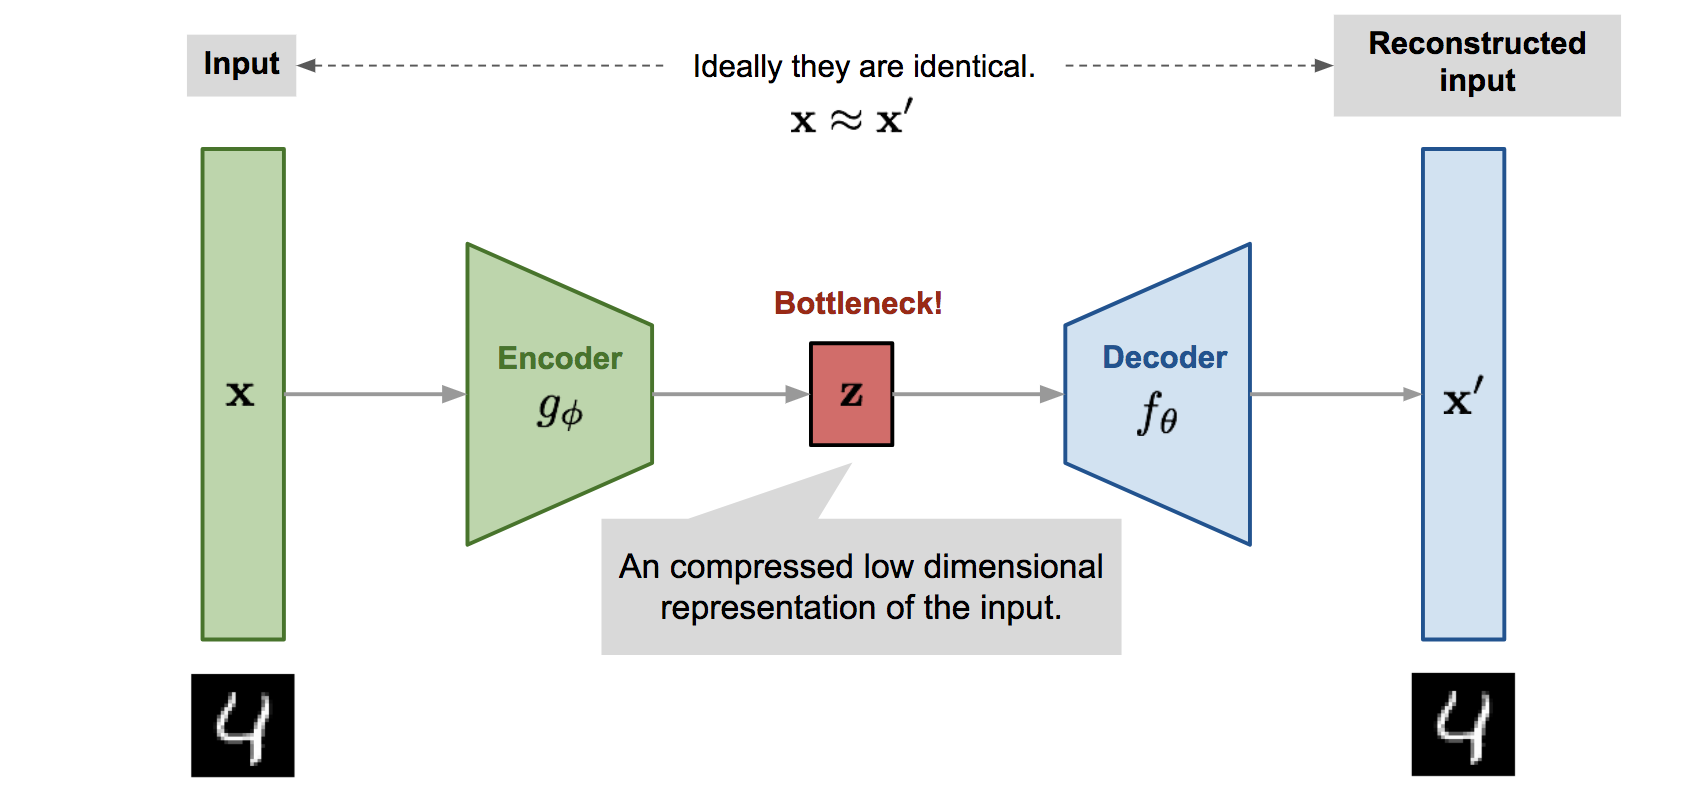
\includegraphics[scale=0.4]{autoencoder-architecture.png}}
\def\paratrick{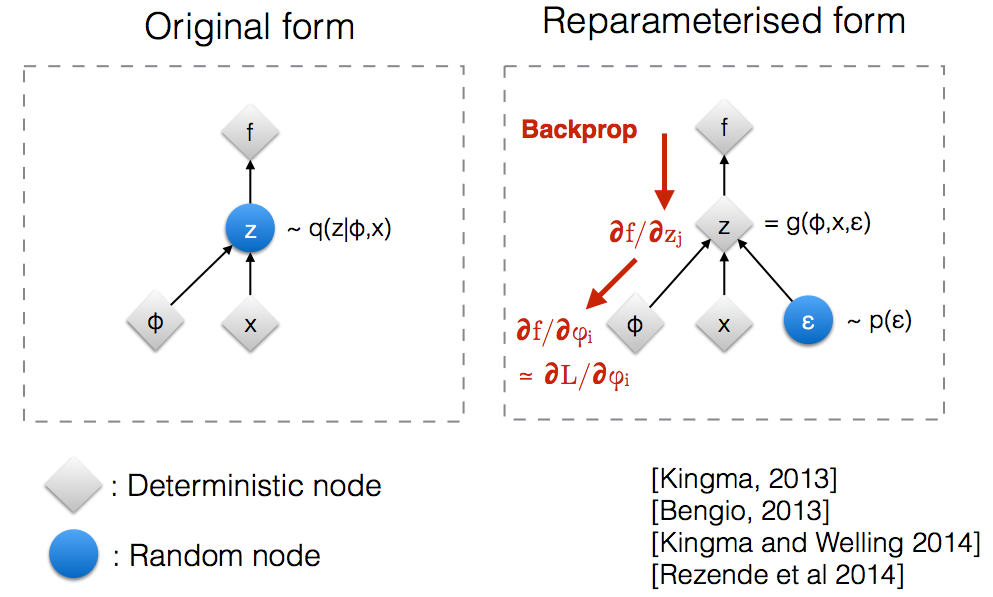
\includegraphics[scale=0.4]{para_trick.png}}
\def\GAN{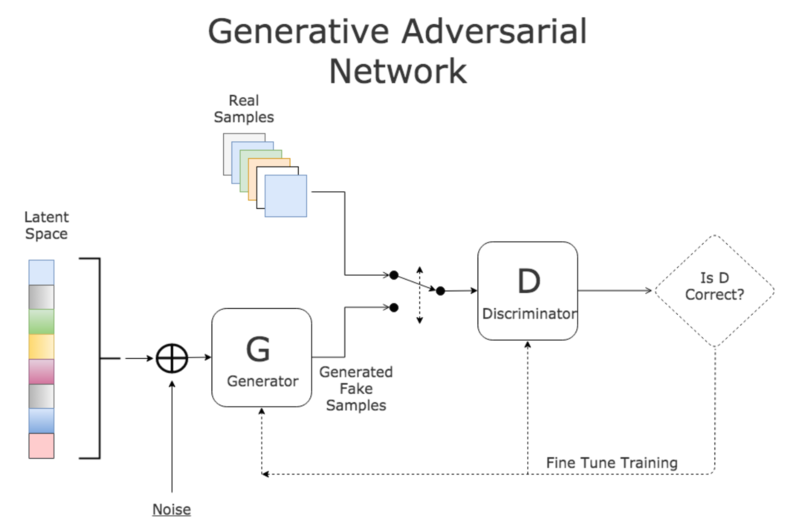
\includegraphics[scale=0.4]{GANs.png}}
\def\GAILExperiments{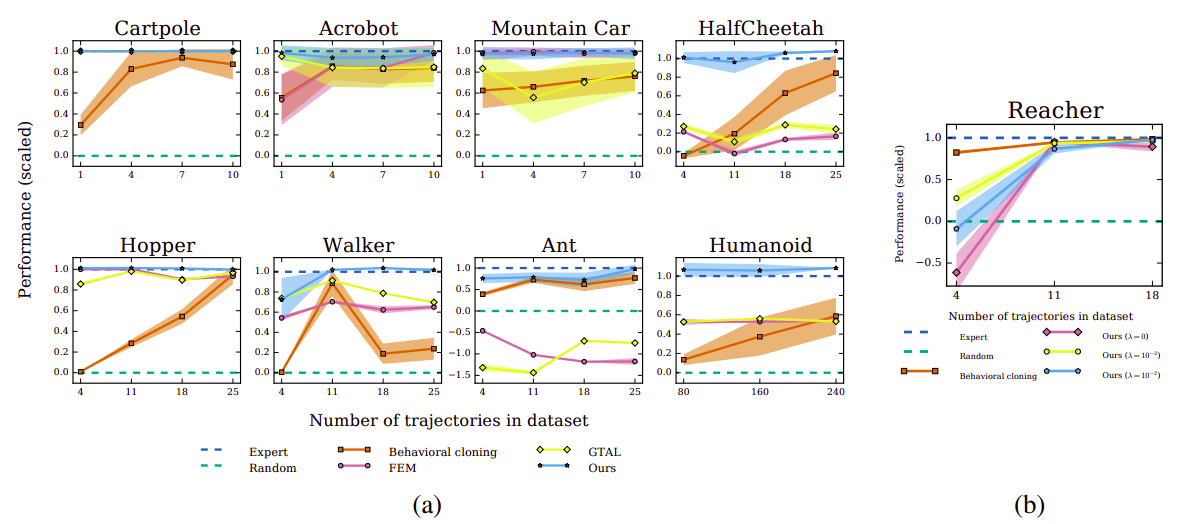
\includegraphics[scale=0.4]{GAIL_exps.png}}
\def\SIGARL{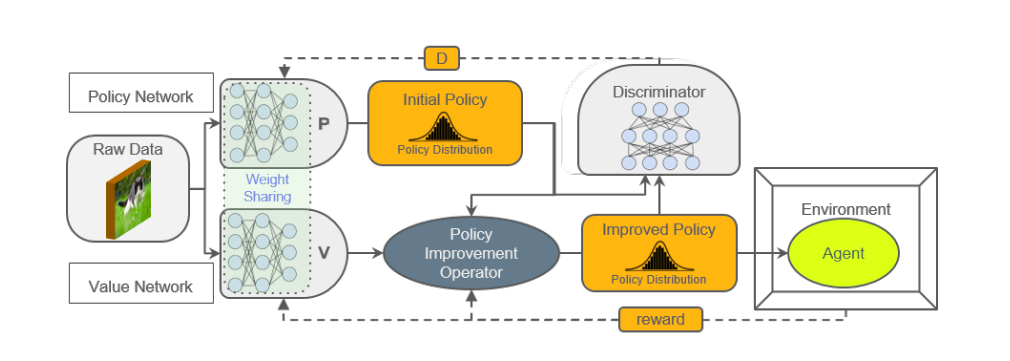
\includegraphics[scale=0.5]{SI_GARL.png}}

\def\RL{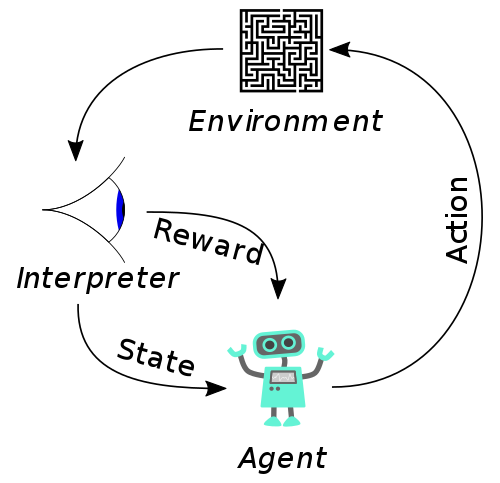
\includegraphics[scale=0.5]{Reinforcement_learning_diagram.png}}
%%%%%%%%%%%%%%%%%%%%

\begin{document}

%Con queto comando si pu� cambaire il modo in cui verranno nominate le
	%figure. Di default � "Figura", qui viene cambiato in "Fig."
	%\renewcommand{\figurename}{Fig.}

	% === Frontespizio =======================================
	% formato della pagina: l'argomento empty sta ad indicare che sia le linee
	% di testa che quelle di coda sono vuoti e non hanno numeri di pagina
	\pagenumbering{roman}
	% Frontespizio: mediante il comando input si legge il frontespizio
	%%%%%%%%%%%%%%%%%%%%%%%%%%%%%%%%%%%%%%%%%%%%%%%%%%%%%%%%%%%
% Frontespizio

% vspace serve ad aggiungere extra spazio verticale
% em sta ad indicare la grandezza della lettera M maiuscola

% Large indica una dimensione del font di 14.4 pt
% large indica una dimensione del font di 12 pt
% normalsize indica una dimensione del font di 10 pt

% vfill inserisce sufficiente spazio binaco verticalmente per fare in modo che il
% sopra e il sotto del testo siano allieneati col margine superiore e inferiore

\hypersetup{pdftitle={Usage example of the Sapthesis class for a Laurea Magistrale thesis in English},pdfauthor={Milad Kiwan}}

% Remove in a normal thesis
%\definecolor{gray}{gray}{0.4}
\definecolor{black}{rgb}{0.0, 0.0, 0.0}
\newcommand{\bs}{\textbackslash}

% Commands for the titlepage
\title{State Of Art Of Generative Models in robotics\\ Applications\\ Master thesis in engineering in computer science}
\author{Milad Kiwan}
\IDnumber{1164659}
\course{Ingegneria Informatica}
\courseorganizer{Facolt\`{a} Ingegneria dell'informazione, informatica e statistica}
\AcademicYear{2019/2020}
\copyyear{2020}
\advisor{Prof. Daniele Nardi}
\advisor{Dr. Francesco Riccio}
%\coadvisor{Dr. Nome Cognome}
\authoremail{miladkiwan@hotmail.com}

\examdate{20 April 2020}
\examiner{Prof. Lenzerini Maurizio}
\examiner{Prof. Nardi Daniele}
\examiner{Prof. Giorgio Grisetti}
\examiner{Prof. Comminiello Danilo}
\examiner{Prof. Massimo	Mecella}
\examiner{Dr. Scardapane Simone}
\examiner{Dr. Anagnostopoulos Aristidis}
\versiondate{\today}


\maketitle

%\clearpage{\pagestyle{empty}\cleardoublepage}

%%%%%%%%%%%%%%%%%%%%%%%%%%%%%%%%%%%%%%%%%%%%%%%%%%%%%%%%%%%
%% Scheda Interna
%
%\begin{titlepage}
% \begin{center}
%     \includegraphics[width=6cm]{logob}\\
%     \vspace{1em}
%     {\Large \textsc{Universit� degli studi di Roma "La Sapienza"}}\\
%     \vspace{1em}
%     {\Large \textsc{Facolt� di Ingegneria}}\\
%     \vspace{2em}
%     {\normalsize Tesi di Laurea in}\\
%     \vspace{1em}
%     {\Large \textsc{Ingegneria Elettronica}}\\
%     \vspace{5em}
%     {\LARGE \textbf{Interazione uomo-robot mediante comandi gesturali e vocali}}\\
% \end{center}
%
%\vskip 2.5cm
%  \begin{center}
%    \begin{tabular}{l c c c c c c l}
%      \large \textbf{Relatore} & & & & & & & \large \textbf{Candidato} \\[0.2cm]
%      \large{Prof. Alessandro De Luca} & & & & & & & \large{Emanuele Magrini}\\[0.4cm]
%       \large \textbf{Correlatore} & & & & & & & \\[0.2cm]
%      \large{Dott. Fabrizio Flacco}& & & & & & & \\
%    \end{tabular}
%  \end{center}
%
%\vskip 2cm
%\begin{center}
%{\normalsize Anno Accademico 2011/2012}
%\end{center}
%\end{titlepage}
\clearpage{\pagestyle{empty}\cleardoublepage}

%%%%%%%%%%%%%%%%%%%%%%%%%%%%%%%%%%%%%%%%%%%%%%%%%%%%%%%%%%%
% Dedica

\vspace{5em}
% \begin{flushright}
% {\Large \textit{to my family and friends}}
% \end{flushright}

\pagestyle{empty}
	
\begin{center}
	%\thispagestyle{empty}
	%\vspace*{\fill}
%{\em To my both colleague and wife, Maram, \\ \qquad \qquad \quad  and to my daughter, Yafa.}
	%{\em To my family.}
	{\em Dedication.}
	%\vspace*{\fill}
\end{center}

%\begin{flushright}
%\vspace*{\fill}
%	To my beloved Mara
%	\vspace*{\fill}
%\end{flushright}

\clearpage{\pagestyle{empty}\cleardoublepage}
	%%%%%%%%%%%%%%%%%%%%%%%%%%%%%%%%%%%%%%%%%%%%%%%%%%%%%%%%%%%
% Abstract
\pagestyle{fancy}

\providecommand{\keywords}[1]{\textbf{Keywords:} #1}

\chapter*{Abstract}
\addcontentsline{toc}{chapter}{Abstract}

\vspace{-30 pt}



\keywords{\textit{Generative models, Generative Adversarial Networks, Reinforcement Learning, Variational Autoencoders, Robotics}}\\

This thesis makes an overview on the most used architectures that have been designed to achieve generative models, and show some of the recent frameworks and algorithms in robotics applications that make use of these generative models. It presents as well how these models assisted the existing frameworks like reinforcement learning that had the lead in succession in robotics applications in the last years. The combination between generative models and reinforcement learning in problems like imitation learning and learn from demonstration has led to achieve better performing frameworks. 

\clearpage{\pagestyle{empty}\cleardoublepage}






	%%%%%%%%%%%%%%%%%%%%%%%%%%%%%%%%%%%%%%%%%%%%%%%%%%%%%%%%%%%
% Acknowledgements

\pagestyle{fancy}
\chapter*{Acknowledgements}
\addcontentsline{toc}{chapter}{Acknowledgements}

Firstly, I would like to express my sincere gratitude to my teacher and advisor Prof. Daniele Nardi and his assistent Francesco Riccio for the sustained support of my masters study and related research, motivation, and immense knowledge. 

\vspace{5pt}
Also, I would like to thank all my friends for their motivation and nice refresh breaks during the day. 

\vspace{5pt}
A big thanks to my parents for their endless encouragement, support, and patience for being far from them.

\clearpage{\pagestyle{empty}\cleardoublepage}


\tableofcontents
\clearpage{\pagestyle{empty}\cleardoublepage}

%\listoffigures
 
%\listoftables

\pagenumbering{arabic}

%%%%%%%%%%%%%%%%%%%%%%%%%%%%%%%%%%%%%%%%%%%%%%%%%%%%%%%%%%%
% Introduction
%\clearpage{\pagestyle{empty}}

\pagestyle{fancy}  
\chapter*{Introduction}
\addcontentsline{toc}{chapter}{Introduction}
\vspace{5 pt}
There is an immense effort in machine learning and statistics to develop accurate and scalable probabilistic models of data. Such models are called upon whenever we are faced with tasks requiring probabilistic reasoning, such as prediction, missing data imputation and uncertainty estimation; or in simulation-based analyses, common in many scientific fields such as genetics, robotics and control that require generating a large number of independent samples from the model. The benefit of employing a generative model lies in its wide applicability to the problem of inference. For example, many robotic tasks include the problem of evaluating the likelihood of an observation of the environment given some piece of relevant information, such as the location of the camera, a particular object model hypothesis, or even raw images. However, generative models in robotics are used to solve various issues faced during the implementation of applications in robotics field to design intelligent machines that can help and assist humans in their day-to-day lives. Such as learn from demonstrations or sometimes called imitation learning, which is a paradigm for enabling robots to autonomously perform new tasks, help reinforcement learning to learn from high-dimensional state space, lean wild set of tasks, and improve polices either with or without demonstrations. The lack of data as well is one of the main efficiency and stability is one of the main challenges in end-to-end methods like those of\textit{ \textacutedbl reinforcement learning\textgravedbl.} It is hard to talk about robotics without mention reinforcement learning, which as a field, has had the major success in past few years. RL offers to robotics a set of tools and algorithms that can assist to design complicated robotic behavior to achieve sophisticated tasks. More recently, another field in machine learning that had the lead in success well as is\textit{ \textacutedbl Generative Adversarial Networks\textgravedbl} this great idea of gaming networks, invented by Ian Goodfellow, has been exploit in RL to achieve more complicated frameworks that, as we will see later in this work.
\\During this work we will talk about the main techniques and algorithms used to perform generative models that have assisted the robotics applications to achieve the respective tasks, and go through some of the frameworks and papers that we deemed most interesting, and showed the importance role the generative modeling plays in the most recent robotics applications. Afterward we will discuss these frameworks explaining their functioning and how the generative models were employed to become useful in the various settings. Then we will show the results obtained from this employment, and argue the effects and the limits on these applications. At the end we will talk about the conclusions extracted during the extension of this survey, and offer some thoughts about how might the generative models in robotics extend and where would be the direction of the future works.


\clearpage{\pagestyle{empty}\cleardoublepage}

%\part{Part I}
%%%%%%%%%%%%%%%%%%%%%%%%%%%%%%%%%%%%%%%%%%%%%%%%%%%%%%%%%%%
% Chapter1


\pagestyle{fancy} 
\chapter{Background}
\label{cha:1}
\vspace{1cm}

\section{Variational Auto-Encoder (VAE) Structure}
\label{cha:VAE}
One of the reasons for which the generative models have been employed in different type of applications is the powerful and utility of VAE, where they are used to either solve issues in AI like image reconstruction and generation, achieve better results, reduce the computational complexity due to the high dimensionality of the data, find latent space, reduce dimensionality, extract and represent features or learn density distribution of the dataset. In this session it is given an overview on how a VAE network is structured and what are the main techniques applied to make it useful to each of the issues just mentioned.\\
Before starting to talk about the usage VAEs, it is mandatory to go through the structure of the auto-encoder which is essentially a neural network with a bottleneck in the middle Fig~\ref{fig:autoencoder} designed to reconstruct the original input in an unsupervised way, in other words, it learns an identity function by first reducing the dimension of the data to the bottleneck so as to extract more efficient and compressed representation. Surprisingly The idea was originated in the 1980s, and later promoted by the seminal paper by~\cite{hinton2006reducing}.

\vspace{0.3cm}
The Auto-Encoder consists of tow connected networks that could be any kind of neural networks (convolutional, or multi-layer perceptron etc) depends on the data it has to deal with, which are:
\begin{itemize}
	\item Encoder network: gets the high-dimension input and transform it to into a low-dimension code in the bottleneck, or we can call it representation, latent or features as well again depends on what the usage are we making of the auto-encoder.
	\item Decoder network: gets the output of the encoder and does essentially the inverse process, or we can say reconstruct the data, likely with larger and larger layers to the last one that outputs the reconstructed original data.
\end{itemize}

\begin{figure}
	\centerline
	\autoencoder
	\caption{Autoencoder}
	\label{fig:autoencoder}
\end{figure} 

We can see already how the auto-encoder networks can give us an efficient way to  impressively represent the data and in lower dimension. So the accomplishment of solutions for the problematics we talked about at beginning of this session, is all about about how we build the bottleneck layer or what will call from now on vector $z$. The VAE~\cite{kingma2013auto} basically is an auto-encoder but the structure of vector $z$ is quite different. For instance what if we need to map the input into a probability distribution $q_{\theta}$ instead of a fixed vector $z$, where $q_{\theta}$ is parameterized by $\theta$, from which we sample or generate $z$, this is what make the VAE to be recognized as a generative model. Where the training is regularized to avoid eventual overfitting  that might occur with auto-encoder architecture and ensure that the distribution $q_{\theta}$ has good parameters to enable the generative process. The way that makes the encoder to be able to produce $q_\theta$ is by composing the bottleneck or the output of a mean $\mu$ and a covariance matrix $\Sigma$ the problem here is that nothing would prevent the this distribution to be extremely narrow, or effectively a single value. To escape the issue, the Kullback-Leibler (KL) divergence-which measures the distance between tow distributions- is introduced  between the distribution produced by the encoder $q_{\theta}(z \mid x_i)$ and a unit Gaussian distribution $p(z)$(mean $0$, covariance matrix is the identity matrix) and tell us how much information is lost when using q to represent p, this KL divergence is then introduced as a penalty to the loss function li, which consists of another term as well that is the expected negative likelihood of the $i$-th datapoint $x_i$ as follow:


\begin{equation}
l_i(\theta,\phi)=-E_{z\sim q_\theta (z\mid x_i)}[\log_{p_\phi}(x_i \mid z)]+KL(q_\theta (z\mid x_i)||p(z))
\label{eq:VAE_loss}
\end{equation}
Where $z$ is sampled from $q_\theta$ and $\phi$ the decoder parameters, the purpose of the first term in poor words mean \textacutedbl how much the decoder output is similar to original datapoint $x_i$\textgravedbl. It intuitively leads the decoder to learn to reconstruct the data. The last important part left to talk about is the training one, we can use the gradient descent to optimize the loss with respect to the parameters of the encoder and decoder $\theta$ and $\phi$ respectively. For stochastic gradient descent with step size $\rho$, the encoder parameters are updated using $\theta=\theta-\frac{\partial l}{\partial \theta} $  and the decoder is updated similarly.



\subsection{Reparameterization Trick:}
\label{cha:VAE_REparam}
As we can notice at this point that there would be a problem doing the backpropagation step of the gradient descent optimizer, because it does not go through the random node z, therefore we have to implement some trick to circumvent this issue. The reparameterization trick~\cite{kingma2013auto} is essentially done by introducing an auxiliary variable (noise) $\varepsilon$ that allows us to reparameterize $z$ in a way that allows backpropagate to flow through the deterministic nodes as shown in Fig.~\ref{fig:paratrick}, we are basically expressing the random variable $z$ as a deterministic 

\begin{figure}
	\centerline
	\paratrick
	\caption{reparameterization trick}
	\label{fig:paratrick}
\end{figure} 

\section{Gaussian Mixture Models (GMMs) structure and learning algorithm}

\label{cha:GMM}
GMM is a probabilistic model for representing normally distributed subpopulations within an overall population. Mixture models in general don't require knowing which subpopulation a data point belongs to, allowing the model to learn the subpopulations automatically. Since subpopulation assignment is not known, this constitutes a form of unsupervised learning. GMMs have been used for feature extraction from speech data, and have also been used extensively in object tracking of multiple objects, where the number of mixture components and their means predict object locations at each frame in a video sequence.
The model is parameterized by two types of values, the mixture component weights are defined as $\theta_k$ and the component means $\mu_k$ and variances $\sigma_k$ or covariances (for the multivariant case) $\Sigma$, the mixture component weights has a constraint that is:  $\sum_{i=1}^{K} \phi_i = 1$ so that the total probability distribution normalizes to 1. The numerical technique used to maximize the likelihood estimation is the Estimation maximization (EM) which consists of tow steps:

\begin{itemize}
	\item	 E-step: consist of calculating the the expectation of the component assignments $P(C_k | x_i)$ for each data point $x_i \in X$ given the model parameters $\phi_k$,  $\mu_k$, and $\sigma_k$.
\end{itemize}
\begin{itemize}
	\item	M-step: which consists of maximizing the expectations calculated in the E step with respect to the model parameters. This step consists of updating the values $\phi_k$,  $\mu_k$, and $\sigma_k$.
\end{itemize}
The entire process iteratively repeats until the algorithm converges, before it starts some initializations are made as follows:
Randomly assign samples without replacement from the dataset $X={x_1, ..., x_N}$, to the component mean estimates $\mu_1,..., \mu_k$. E.g. for K=3 and N=100, set $\mu_1= x_{45}$, $\mu_2 = x_{32}$, $\mu_3 = x_{10}$. 
Set all component variance estimates to the sample variance 
$\sigma_1^2,...,\sigma_k^2=\frac{1}{N}\sum_{i=1}^{K} (x_i -\hat{x})^{2}=1$, where $\hat{x}=\frac{1}{N}\sum_{i=1}^{N}(x_i)$ is the sample mean.
Set all component distribution prior estimates to the uniform distribution  
$P(C_k) = \phi_1,..., \phi_k  = \frac{1}{K}$
while the E-step computes the probability that $x_i$ is generated by component $C_k$:
\begin{equation}
p(C_j \mid x_i ) = \frac{ p(x_i \mid C_j)p(C_j) }{p(x_i)} = \frac{p(x_i \mid C_j)p(C_j)}{\sum_ip(x_i \mid C_j)p(C_j)}
\label{eq:}	
\end{equation}

which will be used in the M-step where the parameters are updated as follow:	

\begin{align}
\mu_j&=\frac{ \sum_{i} p(C_j \mid x_i )x_i}{\sum_{i} {p(C_j \mid x_i )}} \\
\sigma_j^2 &=\frac{\sum_{i}{p ( C_j \mid x_i)}  (x_i - \mu_j) (x_i - \mu_j)^T} {\sum_{i} {p(C_j \mid x_i )}} \\
p ( C_j ) &= \frac{ \sum_{i} p(C_j \mid x_i )}{N}
\end{align}

\begin{figure}
	\centering
	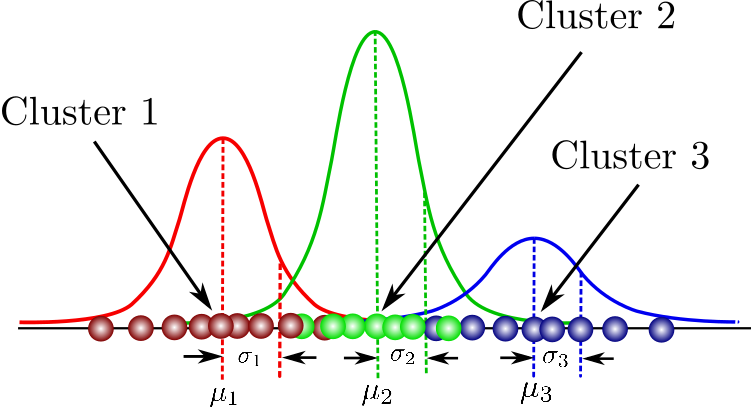
\includegraphics[scale=0.3]{Figures/GMM}
	\caption{}
	\label{fig:GMM}
\end{figure}

\vspace{10pt} 
Originally GMM is employed for classification and clustering tasks, but as we can deduce that it is also a suitable model when recovering the distribution of the data is needed, since it can produce more complexed distribution composed of jointed k gaussians as in Fig.~\ref{fig:GMM}, for example if we have different sources from which the data is provided. Back to our main argument, GMM has been used in several robotics applications, like in Gaussian Mixture Model for Robotic Policy Imitation~\cite{pignat2019bayesian} where different robots had to learn from few amount of demonstrations to complete various tasks such as avoid obstacles, or insert a peg in a moving hole. This approach (GMM) illustrates the advantages of learning a distribution of policies instead of trajectories and can be used in a variety of tasks. On the other hand in some work as in~\cite{zhang2016robot} the GMM was benefited in robot obstacle avoidance learning as a base for a generative model, to generate trajectories, by Gaussian Mixture Regression (GMR), The trajectory obtained not only can avoid obstacles but also can be executed by robots due to its good smooth property. The same idea of~\cite{zhang2016robot} was implemented in~\cite{reiley2010motion} in which GMM encodes the expert\textquotesingle s underlying motion structure. GMR is then used to extract a smooth reference trajectory to reproduce a trajectory of the task. This GMM/GMR generative model was trained on expert data, then tested by classifying the generated trajectories  to be either coming from expert, intermediate, or novice surgeons. The classification algorithm Hidden Markov Models (HMMs) trains three (expert, intermediate and novice) from five new unseen trials for each skill level. The results of the classifier show that each trajectories generated by GMM/GMR are closest to the expert model. To conclude this session it is right and proper to say that the use of GMM has remarkable impact to improve the model performance in presence of lack of data issue.


%\vspace{1cm}
\section{Reinforcement Learning RL}

\label{cha:RL}
This field of machine learning deals with how an agent ought to behave in an environment in order to maximize the reward. It differs from supervised learning in not needing of labeled input/output pairs and from unsupervised learning in getting guidance from the environment by performing actions and learning from the errors or rewards. Typically the environment take the form of a Markov Decision Process (MDP) is a mathematical system used for modeling decision making. We use a tuple (S, A, P, R, $\gamma$) to define a MDP. Where S denotes the state space, a finite set of states. A denotes a set of actions the actor can take at each time step t. P denotes the probability that taking action a at time step t in state st will result in state $s_{t+1}$. $R_a(s,\acute{s})$ is the expected reward from taking action a and transitioning to $\acute{s}$. $\gamma \in [0, 1]$ is a discount factor, to discount the future reward. The general diagram of Reinforcement learning is shown in Fig.~\ref{fig:RL}
\begin{figure}
	\centerline
	\RL
	\caption{Reinforcement learning diagram}
	\label{fig:RL}
\end{figure} 
\vspace{0.3cm}
There are tow notions about the environment where the algorithm that implement RL that should be mentioned which are:
\begin{itemize}
	\item \textacutedbl model-based\textacutedbl algorithms: who are employed when the environment is a priori known, in other words, when we know the transition probability matrix P between states, so the agent can make predictions about the next state and reward before it takes each action.
\end{itemize}
\begin{itemize}
	\item \textacutedbl model-free\textacutedbl algorithms: for which there is no assumption about the world.
\end{itemize}
While about the techniques the algorithm uses to lean the policy are divided as follow:
\begin{itemize}
	\item \textquotedblleft Off-policy\textquotedblright: is that it updates its Q-values using the Q-value of the next state s\textasciigrave and the greedy action a\textasciigrave. In other words, it estimates the return (total discounted future reward) for state-action pairs assuming a greedy policy were followed despite the fact that it is not following a greedy policy.
\end{itemize}
\begin{itemize}
	\item \textquotedblleft On-policy\textquotedblright: is that it updates its Q-values using the Q-value of the next state s\textasciigrave and the current policy\textasciigrave{s} action a. It estimates the return for state-action pairs assuming the current policy continues to be followed.
\end{itemize}

In this work, all the algorithms referred to are model-free since in robotics applications usually the software agent can not make any prediction about the environment, and no assumption is made whether it is on-policy or off-policy.

\vspace{0.3cm}
Going through the various algorithms of RL you can realize that in most cases there is not best algorithm, it all depends on task, environment, discrete or continuous spaces, and the data itself and its size. During my studies I have implemented different algorithms in RL which are Deep Q Learning (DQN), Deep Deterministic Policy Gradient (DDPG) and Trust Region Policy Optimization (TRPO). Basing on my modest experience I realized is that as long as we have simple and well-defined environment, picking the algorithm who is more fit to the task taking into account the domain spaces of actions and states, eventually will get good results, the agent will learn a close-to-optimal policy to behave in the environment. But when the task (policy) to be learned is more complicated in respect of the lack of resources and data and its quality, then it is more than convenient making some process on the input data to make the learning policy process more efficient computationally and of course in terms of results which are our aim first of all, for example find the latent space of the data, or define a probability distribution that describe the dataset. That what I found out while doing my survey about generative models in robotics, where RL is strongly present regardless on which algorithm has been employed, actually most of times the algorithm used was not mentioned. 

\section{Generative Adversarial Networks (GANs)}

\label{cha:GANs}
Generative adversarial networks (GAN) is algorithmic architecture that uses two neural networks, pitting one against the other (thus the \textacutedbl adversarial\textgravedbl) in order to generate new, synthetic instances of data that can pass for real data. They are used widely in image generation, video generation and voice generation. it was introduced firstly by~\cite{goodfellow2014generative} to create a new framework for estimating generative models via an adversarial process that corresponds to tow-player game,
the tow networks could have arbitrary architecture and they are trained simultaneously, one neural network, called the discriminator, is designed as classifier network to evaluate the authenticity  distinguishing between fake and real data instances, while the other one, called generator, is trained to generate data as close to the authentic ones. Meanwhile, the generator is creating new, synthetic instances that it passes to the discriminator. It does so in the hopes that they, too, will be deemed authentic, even though they are fake. The goal of the generator is to generate passable instances to lie without being caught. The goal of the discriminator is to identify those coming from the generator as fake. GANs are a clever way to train a generative model in the same manner of a supervised learning problem.\\
To describe the GAN algorithm Fig.~\ref{fig:GAN} it is possible to start from either the generator, or the discriminator, because as mentioned in the previous section it corresponds to a tow-player game, like in chess, conventionally the while starts, but even if black starts that does not change the essence of the game. However, let's start with the more interesting one with is the generative model.\\
\begin{figure}
	\centerline
	\GAN
	\caption{GAN Architecture}
	\label{fig:GAN}
\end{figure} 
The generator model takes a fixed-length random noise vector as input and generates a sample in the domain. The vector is drawn randomly from a Gaussian distribution, and the vector is used to seed the generative process. This vector space is referred to as a latent space, or a vector space comprised of latent variables. Latent variables, or hidden variables, are those variables that are important for a domain but are not directly observable. It is often referred to latent variables, or a latent space, as a projection or compression of a data distribution. That is, a latent space provides a compression or high-level concepts of the observed raw data such as the input data distribution. In the case of GANs, the generator model applies meaning to points in a chosen latent space, such that new points drawn from the latent space can be provided to the generator model as input and used to generate new and different output examples, 
after training, the generator model is kept and used to generate new samples. Sometimes, the generator can be repurposed as it has learned to effectively extract features from examples in the problem domain. Some or all of the feature extraction layers can be used in transfer learning applications using the same or similar input data. \\

The Discriminator Model takes an example from the domain as input (real or generated) and predicts a binary class label of real or fake (generated).The real example comes from the training dataset. The generated examples are output by the generator model. The discriminator is a normal (and well understood) classification model. After the training process, the discriminator model is discarded as we are interested in the generator.\\
The generator and the discriminator have different training processes, and it proceeds in alternating periods:
\begin{enumerate}
	\item The discriminator trains for one or more epochs.
	\item The generator trains for one or more epochs.
	\item Repeat steps 1 and 2 to continue to train the generator and discriminator networks.
\end{enumerate}

Indeed, as the generator improves with training, the discriminator get worse, because it becomes more difficult to recognize the authentic instances rather than the generated one, which means in accuracy terms that if the generator succeeds perfectly then the discriminator has a 50\% accuracy, same as flipping a coin to predict the label of the current instance.
This progression poses a problem for convergence of the GAN as a whole: the discriminator feedback gets less meaningful over time. If the GAN continues training past the point when the discriminator is giving completely random feedback, then the generator starts to train on junk feedback, and its own quality may collapse, which produces limited varieties of samples. Contrarily. If the discriminator gets too successful that the generator gradient vanishes and learns nothing.
Anyways, training GANs is noted as hard to obtain but still there several techniques to make the training more stable, which are out of the boundaries of this work. GANs try to replicate a probability distribution. They should therefore use loss functions that reflect the distance between the distribution of the data generated by the GAN and the distribution of the real data. Of course, there are tow loss functions for each of the tow networks as introduced in~\cite{goodfellow2014generative}, the generator tries to minimize the following function while the discriminator tries to maximize it:
\begin{equation}
E_x[\log{D(x)}] + E_z[\log{(1-D(G(z)))}]
\label{eq:GAN_loss}
\end{equation}

where $D(x)$ is the discriminator's estimate of the probability that real data instance x is real.
$E_x$ is the expected value over all real data instances. $G(z)$ is the generator's output when given noise z. $D(G(z))$ is the discriminator's estimate of the probability that a fake instance is real.
$E_z$ is the expected value over all random inputs to the generator (in effect, the expected value over all generated fake instances $G(z)$). The formula derives from the cross-entropy between the real and generated distributions. Since the generator can not directly affect $\log{D(x)}$ so, for the generator, minimizing the loss is equivalent to minimizing $log(1 - D(G(z)))$.


\clearpage{\pagestyle{empty}\cleardoublepage}
%\part{Part II}
%%%%%%%%%%%%%%%%%%%%%%%%%%%%%%%%%%%%%%%%%%%%%%%%%%%%%%%%%%%
% Chapter2


\pagestyle{fancy} 
\chapter{Generative Modeling in Robotics}
\label{cha:2}
\vspace{1cm}

\section{Employment of VAEs and DNNs in generative models for robotics}
\label{sec:VAE_generative}
Lets go now through some papers to see where and how the VAEs have been employed and show their effectiveness in various applications of generative models in robotics. The first one~\cite{eslami2016attend} where a framework called by the authors \textsl{Attend, infer, repeat (AIR)} the VAE structure here is quite different that the encoder was implemented as a Recurrent Neural Network (RNN), since its purpose is to learn to detect and generate objects, specifically “where is the objects, what are they and how many are they”. The additional recurrence to the structure is basically to detect how many objects are present in the input data. Experiments were designed initially on 2D data particularly on multiple MNIST digits, and reliably the model were able to detect and generate the constituent digits from scratch, it shows advantages over state-of-art generative models computationally and also in terms of generalization to unseen datasets. Other Experiments on 3D datasets, considering scenes consisting of only one of three objects: a red cube, a blue sphere, and a textured cylinder. The network accurately and reliably infers the identity and pose of the object, on the other hand, an identical network trained to predict the ground-truth identity and pose values of the training data has much more difficulty in accurately determining the cube\textquotesingle s orientation.\\

Moreover, in robotics, grasping and manipulation of various objects is a critical and challenging problem,~\cite{veres2017modeling} has proposed another concept referred to as the grasp motor image (GMI) that combines object perception and a learned prior over grasp configurations, to synthesize new grasps to apply to a different object. At the core of GMI is the autoencoder structure, taking advantage of Deep  Learning (DL), particularly building both encoder and decoder as Convolutional Neural Networks (CNN). The approach followed is intuitive: based on
perceptual information about an object, and an idea of how an object was previously grasped, collecting a object/grasp pair dataset of successful, cylindrical precision robotic grasps using the V-REP  simulator~\cite{rohmer2013v}, and object files provided by~\cite{kleinhans2015g3db} on a simulated “picking” task. The VAE was trained on this dataset to generate grasps for novel objects. GMI integrates
perceptual information and grasp configurations using deep generative models. Applying it to a simulated grasping task, has demonstrated the capacity of these models to transfer learned knowledge to novel objects under varying amounts of available training data.\\

Moreover, a novel data generation pipeline for
training a deep neural network (DNN) approach was introduced in Domain randomization and generative models for robotic grasping~\cite{tobin2018domain}, that perform the grasp planning for randomized objects domain. The model architecture of this paper is composed of tow parts that are trained separately, the second part is
grasp evaluation model $f$ that acts as a classifier taking as input a single observation image from the robot and outputs a single scalar value corresponding to the likelihood of success of that grasp returned from the planner. While the more interesting part is first one which is the grasp planning module $\gamma(I) = \beta \circ \alpha(I)$ Where $\beta$ consists of $n$ (the dimensionality of the grasp) small NNs, each of them takes as input a representation of the image $s$ and outputs a softmax over possible values of $g$ as follows:
\begin{equation}
\beta(s)(g) = \displaystyle \prod_{i=1}^{n}\beta_i(g_1,...,g_n,s)
\end{equation}
In other words, what actually the planner outputs is a probability distribution over possible grasps.

It initially takes as input 2 images and putts a sto . employ several NNs each returns 

\section{Exploitation of VAE and GMM in RL}
As mentioned in the previous section, most of the time applying RL algorithm directly on high-dimensional data does not lead to a good performance, so in the kind of situation it is advantageous to make use of the techniques that permit to reduce the dimensionality by representing the data in more suitable way.\\
One of the frameworks I went through has exploit both VAE and GMM to neatly which makes it feasible to fit the dynamics even when the number of samples is much lower than the dimensionality of the system. this what~\cite{finn2016deep} does, where initially RL algorithm run on robot with initial random policy to collect N (5 for that experiment) samples, then use them to fit GMM to learn the environment dynamics  or the policy controller without vision but using only the robot’s configuration as the state. In a second phase a VAE is trained to encode image dataset with unsupervised learning to produce a low-dimensional bottleneck vector that is a natural choice for learned feature representation or feature points for each image that concisely describes the configuration of objects in the scene, the interesting part of this VAE is that it is forced to encode spatial features rather than values. This is obtained  basically by applying spatial soft-max activation function that consists of tow operations on the last convolutional layer of the encoder as follow:
\begin{equation}
s_{cij} = \frac {e^{\frac{a_{cij}}{\alpha}}}
{\sum_{\acute{i}\acute{j}} e^{ \frac {a_{c \acute{i} \acute{j}}}{\alpha}}}
\end{equation}
where the temperature $\alpha$ is a learned parameter. Then, the expected
2D position of each softmax probability distribution $s_c$ is
computed according to:
\begin{equation}
f_c = (\sum_i i ∗ s_{cij} , \sum_j j ∗ s_{cij} )
\end{equation}
which forms the autoencoder's bottleneck and essentially it is the learned spatial feature point representation, that will therefore be capable of directly localizing objects in the image. The third and final phase of this framework is same as the first one, but the difference here is that the controller is trained on the feature points of the encoder using same trajectory-centric reinforcement
learning algorithm.\\
The experiments of this method showed that it could be used to learn a wild range of manipulation skills that require close coordination between perception and
action, and uses a spatial feature representation of the environment, which is learned as a bottleneck layer in
an autoencoder. This allows us to learn a compact state from high-dimensional real-world images. Furthermore, since this
representation corresponds to image-space coordinates of objects in the scene, it is particularly well suited for continuous control. The trajectory-centric RL algorithm we employ can learn a variety of manipulation skills with these spatial
representations using only tens of trials on the real robot.\\

In another work~\cite{nair2018visual} a RL framework was designed to jointly learns representations and policies from raw sensor inputs that achieve arbitrary goals under this representation by practicing to reach self-specified random goals during training. Here shows up the problem of choosing a suitable goal representations, to deal with this, a goal space \c{G} as to be same as the state space \c{S}. As well the problem of high-dimensional observations such as images arises, to handle it the authors once again the rely on VAE to learn a latent embedding for both \c{G} and \c{S}, by executing a random policy to collect state observation and optimize Eq.~\ref{eq:VAE_loss}, an additional online training has been introduced where the VAE is fine-tuned during the policy training each 3000 environment steps on all of the images observed by the policy, because as the policy improve it might visit new state observations where the VAE is not trained on, this additional training helped the performance of the overall algorithm. The final step is to run the RL algorithm which is a value-based one in this work twin delayed deep deterministic
policy gradients (TD3)~\cite{fujimoto2018addressing} is used, the thing that should be pointed out here that the negative Mahalanobis distance in the latent space were used as a reward function, but it turned out that minimizing this squared distance was equivalent to maximize the probability of the latent goal. This framework for learning general-purpose goal-conditioned policies that can achieve goals specified with target observations.\\


\section{GANs vs VAEs}

VAEs are a probabilistic graphical model whose explicit goal is latent modeling, and accounting for or marginalizing out certain variables as part of the modeling process. They can make good generations, though they are ideal in settings where the latent is important. The VAE naturally collapses most dimensions in the latent representations, and you generally get very interpretable dimensions out, its ability to set complex priors in the latent is also nice especially in cases where you know something should make sense or you have a desired latent distribution. As well as we have seen in section~\ref{sec:VAE_generative}, instead GAN is explicitly set up to optimize for generative tasks, though recently it also gained a set of models with a true latent space. The worry of VAE is that it extend the probability distribution over datapoints that does not make sense, whereas GAN may miss them but as a result for a generative model it looks more reasonable. However it is hard to tell which one is better it all depends on the task, because it is hard measure and test. Speaking of VAEs and GANs, it is therefore appropriate mention the work done in~\cite{rahmatizadeh2018vision} they developed an approach that takes as input images of the environment and outputs the next joint configuration of the robot to execute. combination of VAE-GAN structure and LSTM was composed to build a Robot controller using end-to-end learning from demonstration, where the controller is a LSTM used to generate joint commands to control the robot, and it is based on a GMM, instead of predicting all the outputs (joint configurations), they are factorized into one-dimensional distributions, one for each joint configuration. while the VAE-GAN structure consists of three neural networks . The first network is an encoder that finds the distribution of the data and then sample a latent representation $z=q(z\mid x)$. The second part of the autoencoder is a GAN discriminator that takes a real image or a reconstructed image and tries to predict whether it is real or reconstructed. The objective $E_{GAN}$ is then computed as in eq.~\ref{eq:GAN_loss}. regarding VAE, the objective in eq.~\ref{eq:VAE_loss}is changed  in this paper where the first term $[\log_{p_\phi}(x_i \mid z)]$ is replaced by $E_{GAN}$, plus the reconstruction error where they used mean squared error (MSE) between the extracted features from those images in the third convolutional layer of the discriminator as follows: $E_{rec} = MSE(D_3(x), D_3(\tilde{x} ))$ whereas the normal prior imposed to the latent distribution p(z) to regularize the encoder $E_{prior}=KL(q_\theta (z\mid x_i)||p(z))$ is kept. Finally, the error of the autoencoder network can be described as the sum of errors formulated before: $E_{AE} = E_{GAN}+ E_{rec} + E_{prior}$.\\
The proposed model, as the experiments showed, is very powerful and it does not have any assumption about the task or the shape of objects that are involved in each task. It generated smooth trajectories that follow reasonable path in different situations. This is good since we can train the model on a wide variety of tasks. However, we need large number of demonstrations to successfully learn a single task. At the same time it could be used for a wild variety of tasks given its generalization property acquired from the VAE-GAN structure.

\section{Combination between GANs and RL}

RL is a powerful technique to train an agent to perform a task, so it is capable of achieving that single task specified via its reward function. It an approach that is hard to be scaled to a situation where the agent needs to perform different set of tasks,  such as navigating to varying positions in a room or moving objects to varying locations.~\cite{held2018automatic} has offered an idea that combine RL and GANs that is able to solve this kind of situations, in this framework, instead of learning to optimize a single reward function, an indexed range of reward functions $r^g$ is defined, each goal $g \in G$ corresponds to a set of states $S^g \subset S$, in such way that the goal $g$ is considered to be achieved from any state $s_t \in S$. The policy that should be learned ,given a goal $g$, must perform optimally with respect to $r^g$. The framework uses a simple indicator function to define the reward that gives a measure whether the agent has reached the goal $r^g(s_t, a_t, s_{t+1})=1 \{s_{t+1} \in S^g\}$ where $S^g = \{s_t : d(f(s_t), g)< \epsilon\}$ e $f(·)$ is a function that projects a state into goal space G, $d(.,.)$ is a distance metric, $\epsilon$ acceptable tolerance that determines when the goal is reached. it is also defined a uniform distribution $P_g(g)$ ,although in practice any distribution can be used, over the set of goals $G$ to sample from, so the overall objective function that the authors call it \textit{coverage} will be:
\begin{equation}
\pi^*(a_t \mid s_t, g)= \arg{\max_{\pi}}{E_{g\sim P_g(.)} R^g(\pi) }
\end{equation}
Where $R^g(\pi)$ is the success probability of each goal. Sampling goals from $P_g(g)$ is modified to be uniform only over a set of goals grounding on the level of difficulty, or in better words, Goals of Intermediate Difficulty (GOID):
\begin{equation}
GOID_i := \{ g : R_{min} \leqslant R^g(\pi_i) \leqslant R_{max}\}
\end{equation}
Due to sparsity for the reward function the current policy $\pi_i$ for most goals would not get reward, in the way it will be hard to train the policy, to circumvent this, the sampled goal g should grantee that $\pi_i$ is able to receive some minimum expected return $R_{min}$. On the other hand to prevent the policy keeps training on only some of those goals that get very high reward, the $R_{max}$ restriction is added to make the policy train on the goals who are not mastered yet. $GOID_i$ allows the policy to train on wild coverage objective. that was the first part of the algorithm designed in this framework which is partitioned into three stages. The second stage is the Goal-GAN employment, its generator network is used to generate goals that fall in $GOID_i$, from noise $z$, while the discriminator network distinguish the goals that are in $GOID_i$ from those that are not. a modification has been added to the LSGAN introduced implementation in~\citealp{Mao_2017_ICCV} this modification allows to train
the LSGAN both with positive examples from the distribution we want to approximate and negative examples
sampled from a distribution that does not share support with the desired one this gave the chance to improve the accuracy of the generative model even though it was trained on few positive samples. This adoption was made by introducing a binary label $y_g$ that permit to train on "negative samples" when $y_g = 0$ then optimize the LSGAN objectives:
\begin{align}
\nonumber min_D V(D) &= E_{g \sim pdata(g)}[y_g(D(g)-b)^2 + (1 -y_g)(D(g)- a)^2] + E_{z∼p_z(z)}[(D(G(z))- a)^2]\\ 
max_G V(G) &= E_{z∼p_z(z)}[(D(G(z))- c)^2]
\label{eq:LSGAN_loss}
\end{align}
using $(a = -1$, $b = 1$, and $c = 0)$. \\At each iteration $i$ the algorithm initially sample the noise vector $z$ to generate a goals $G(z)$  that are used train the RL algorithm this time TRPO with AGE is used as in~\cite{schulman2015high} afterwards the is evaluated to assign a label $y_g$ to each goal, and use these labels to train the goal generator and goal discriminator of the GAN following eq.~\ref{eq:LSGAN_loss}. Few experiments have been done to test this method, one of them was a Ant navigation in a maze, in this case the goals generated have tow dimensions $(x,y)$ and it is been discovered that the generated goals were concentrated in some area were the policy is receiving some expected return signals which obviously need improvements, however still the Goal-GAN can shift the distribution of sample goals of the appropriate difficulty dynamically around the origin in a ring growing manner. Similarly another experiment was made on a multi-path point-mass maze here again the generator was able to produce a multi-modal distribution over the appropriate goal of intermediate level of difficulty. In this last experiments, it is been used N-dimensional Point Mass the full state-space of the N-dimensional Point Mass hypercube. However, the Point Mass can only move within a small subset of this state space, also here the performance was good, using the goal-GAN as a generative model even
without this prior knowledge, the Goal GAN discovers the feasible portion of the goal space and generate automatically for the policy that are at the appropriate level of difficulty.\\
One more paper that made use of GAN is Generative Adversarial Imitation Learning (GAIL)~\cite{DBLP:journals/corr/HoE16} where the agent has to imitate an expert behavior, the algorithm make use of the RL algorithm TRPO which at each iteration construct a careful step scheme to update the policy to ensure that the divergence does not occur, simultaneously exploiting the GAN architecture, where the discriminator distinguish between trajectories generated by the generator, in turn, generate trajectories following TRPO, in other words, the generator is the policy to be learned following the lead of the discriminator. Specifically the generator generate a trajectory $\tau_i$ by executing TRPO, then the discriminator updates its parameters $w_i$ to $w_{i+1}$ with the gradient:
\begin{center}
	$E_{\tau_i}[\nabla_w\log{D_w(x)}] + E_{\tau_E}[\nabla_w\log{(1-D_w(G(z)))}]$
\end{center}
afterwards the generator is update function in this paper is composed of tow terms the first is like TRPO algorithm, by finding a trust region in which la policy can move, preventing it of changing too much due to noise in the policy gradient and move it toward expert-like regions of state-action space, and the second term is the casual cross entropy that is used as a cost function or policy regularizer as the following:
\begin{equation}
E_{\tau_i}[\nabla_{\theta}\log{\pi_{\theta}(a \mid s)}Q(s,a)] - \lambda \nabla_{\theta} H(\pi_{\theta})
\label{eq:gail_loss}
\end{equation}
where $\lambda \geqslant 0$ is a hyperparameter and $Q(s,a) = E_{\tau_i}[log{(D_{w+1}(s,a))} \mid s_0=s,a_0 = a]$
The previous iteration repeat until convergence, in other words like in GAN algorithm, it repeats till finding a saddle point $(\pi, D)$ of the expression~\ref{eq:gail_loss} between the tow approximation functions of the policy and the discriminator.\\
The algorithm has been tested on 9 physics-based control tasks, varying from low-dimensional control tasks from the classic RL literature for example cartpole, acrobot, and mountain
car, to difficult high-dimensional tasks such as a 3D humanoid locomotion, solved only recently
by model-free reinforcement learning. the procedure followed for each of these experiments was firstly to generate an expert behavior be running TRPO (not the generator of the GAN of this algorithm) on the true cost function, the algorithm was compared with three baselines such are Behavioral cloning, Feature expectation matching (FEM), Game-theoretic apprenticeship learning (GTAL). All algorithm had the same neural network architecture to train the policy and have been given the same amount of interactions with the environments.

\begin{figure}
	\centerline
	\GAILExperiments
	\caption{(a) Performance of learned policies. The y-axis is negative cost, scaled so that the expert achieves 1 and a random policy achieves 0. (b) Causal entropy regularization λ on Reacher.}
	\label{fig:GAILExperiments}
\end{figure}
As we can see in Fig.~\ref{fig:GAILExperiments} this algorithm produced policies performing better than the other baselines except on the Reacher environment, where behavioral cloning performed excellently even though it suffered on the classic control tasks, while we could see in Fig.~\ref{fig:GAILExperiments}b the effect of causal entropy regularization λ we have met in eq.~\ref{eq:gail_loss}, tuning it has changed the performance of the overall algorithm GAIL on the Reacher task. Instead on the other MuJoCo environments, GAIL has achieved at least $70\%$ of the expert behavior for all datasets, as well as performing much better then the other baselines for on all the tasks.\\
GAIL is not the unique algorithm to take advantage and use of the GAN architecture, Self-Improving Generative Adversarial Reinforcement Learning (SL-GARL)~\cite{liu2019self} as well has developed another framework that once again exploits it to imitate the expert. The general concept repeat itself where the discriminator acts as a classifier and gives a high error values to the initial policies and low error values to the improved ones, while the goal of the generator is to generate policies to minimize the error values. In addition SL-GARL employs a black box improvement policy operator, generally speaking this kind of function may get the computational complexity worse, but in this case it helps to shrink the exploration space and a consumption on computational resources. This operator maps a policy and a state value to an improved policy $ \acute{\pi} = I(\pi, V_\pi)$ that is supposed to be better then the direct output from the policy neural network, because it produces the expert demonstration of the improved policy. The Self-Improving RL algorithm employs tow neural networks one is for evaluating the state value function  $\hat{V}(s,a)=DNN_\theta(s)$ where $\theta$ is the neural network parameters. The second neural network is for the policy estimator defined as $\hat{\pi}(a \mid s,w)$ where $w$ is the neural network parameters, this network will be considered as the generator of the GAN. The loss function at this point is going to be the KL-divergence between the improved policy and the agent one as follows:
\begin{equation}
L_I(w,\theta,s) = D_{KL}[I(\hat{\pi}(\cdotp \mid s,w),\hat{V}(\theta,s))\parallel \hat{\pi}(\cdotp \mid s,w)]
\end{equation}
Hence the update formulas for SI-RL will be:
\begin{align}
\nonumber w_{k+1} &= w_k + \nabla_w L_I(w_k, \theta_k,s) = w_k - I(\hat{\pi}(\cdotp \mid s,w),\hat{V}(\theta,s))\nabla_w \log{\hat{\pi}(\cdotp \mid s,w)}\\
\nonumber \theta_{k+1} &= \theta_k + \nabla_\theta L_I(w_k, \theta_k,s) = \theta_k - I(\hat{\pi}(\cdotp \mid s,w),\hat{V}(\theta,s))\nabla_\theta \log{\hat{\pi}(\cdotp \mid s,w)} + \nabla_\theta {\parallel \hat{V}(\theta,s) - R \parallel}^2
\label{eq:update_SI_RL}
\end{align}
The outputs of these tow networks, The state value $\hat{V}(\theta,s)$ and the initial policy $ \hat{\pi}(\cdotp \mid s,w)$ are then passed to the operator $I$. The inclusion of the GAN was by adding a discriminator which distinguish between improved policy which will interact with the environment and the initial one generated by the policy network, the figure Fig.~\ref{fig:SIGARL} describe the architecture and data flow of the framework. The authors of this paper have evaluated three different algorithms to implement the policy improvement operator:
\begin{itemize}
	\item \textbf{ trust region policy optimization (TRPO):}  which can be used as policy improvement operator directly without any modification, because of the monotonic improvement guaranteed in TRPO
	\item \textbf{Monte Carlo tree search (MCTS):}~\cite{browne2012survey} is a search algorithm that uses randomness for deterministic problems difficult or impossible to solve using other approaches, it is based on tree data structure, it can be used as
	a planning-based police improvement operator. It provides a long term panning ability compared to the policy gradient methods
	\item \textbf{cross entropy
		method (CEM):} Since all policies are parametrized by some network parameters, and the aim is to modify these parameters in such way that the total discount reward is maximized, this method take this problem as a black box with respect to the parameter $\theta$, and it maintains
	a distribution over parameter vectors and moves the distribution
	towards parameters with a higher reward.
\end{itemize}
\begin{figure}
	\centerline
	\SIGARL
	\caption{The architecture of SI-GARL framework. Arrows with solid lines show how the data transfer between modules, and
		those with dotted lines show the feedback signal used to update the networks. The orange blocks represent the internal data.
		The grey circle represents the policy improvement operator seen as a black box}
	\label{fig:SIGARL}
\end{figure}

Both GAN and self-improving procedures show their potential in multiple test domains either against typical deep reinforcement learning (DRL) algorithms like DQN or the actor-critic algorithms like Asynchronous Actor-Critic Agents (A3C).

Since the lack of data is one of the main challenges that RL faces. Recent researches solve the problem resort to supervised learning methods by utilizing human expert demonstrations, or by imitation learning like the previous paper we talked about.


\clearpage{\pagestyle{empty}\cleardoublepage}
%%%%%%%%%%%%%%%%%%%%%%%%%%%%%%%%%%%%%%%%%%%%%%%%%%%%%%%%%%%
% Chapter3


\pagestyle{fancy} 
\chapter{Discussion}
\label{cha:3}
\vspace{1cm}

Going through the different frameworks we have seen in the previous section, we could notice that sometimes the goal of some researches are the same, like to find the probability distribution of data, or to maximize the total returned reward, generate new data instances, but the various authors were making different choices of the available techniques to achieve there goal in solving the task. We could explain these choices by making one step back and have a look on the data. Firstly the question that should be made is \textacutedbl what is the raw data the framework is going to cope with?\textgravedbl. The data we have seen are of different natures like trajectories, images, sensory data, grasp configuration and so on. Posting this question initially leads to figure out what are the space dimensions to deal with, and gives place to additional questions like \textacutedbl should we move to latent space?\textgravedbl in case it is high-dimensional like images. Another main question is \textacutedbl How big is the dataset?\textgravedbl this one is very important impact on the choice to make on the technique to use for the generative modeling, I discovered that when the dataset to base on the not large enough, means that it is more opportune to know probability distribution to generate new data instances from, so the choice of VAEs~\ref{cha:VAE} with reparameterizing trick~\ref{cha:VAE_REparam} in this case should be a good fit. Nevertheless, VAEs struggles to find a complex probability distribution in situations where the dataset is high-dimensional and composed of variables that vary in wild ranges, to overcome this kind of issue the GMM~\ref{cha:GMM} approach may fit better, given the property of GMM to combine $K$ probability distributions components to represent a final probability distribution that fits more efficiently the dataset. Moreover, in human cloning and/or learn from demonstrations tasks, where data are collect by making an expert to behave or execute actions in environment to achieve the goal of the task, this collected dataset is usually small for both learning process of the agent given some demonstrations, or cloning an expert behavior to achieve the required task. In this kind of situations where the amount of data available is not big enough, VAEs still not a good choice unless we follow the idea of moving to the latent space, then VAEs is the best option taking advantage its nice probabilistic formulation they come with as a result of maximizing a lower bound on the log-likelihood. Working in latent space is another approach that can circumvent the high-dimension real-world data. VAE naturally collapses most dimensions in the latent representations, and generally getting very interpretable dimensions out, even though the training dynamics are generally a bit weird. VAEs are used as well to learn the data representation like in~\cite{finn2016deep} which is a reinforcement learning application to robotic manipulation tasks. The authors were interested in knowing the spatial feature representation of the environment, these spatial features are the configurations of objects in the scene. The bottleneck of the autoencoder was modified in such way the spatial representation is learned. VAE has shown its ability as well as a generative model like in~\cite{eslami2016attend} formalizing a framework called \textit{Attend, infer, repeat} for efficient variational inference in latent spaces of variable dimensionality. The key idea of this paper is to treat inference as an iterative process, implemented as a recurrent neural network that attends to one object
at a time, and learns to use an appropriate number of inference steps for each image. VAE as a generative model is able to compete with GAN which is the most interesting idea in machine learning of the last 10 as Yann LeCun, Director of AI Research at Facebook AI claims. GANs is a superior model with respect to VAEs because they are better at generating visual features this superiority conduct to say that the adversarial loss is better than mean-squared loss. The difference that products this superiority is that VAE can spread the probability mass to places it might not make sense, whereas GAN models may never explore. Later, a cooperation between VAE and GAN has been done in~\cite{rahmatizadeh2018vision} mentioned in~\ref{sec:GAN-VAEs} which is one of the most advanced paper I read during this survey, that represent the state of art of robot manipulation tasks. it demonstrated how it is possible to learn complex manipulation tasks from user demonstrations, such as picking up a towel, wiping an object, and depositing the towel to its previous position, entirely from raw images with direct behavior cloning and outputs the joint configuration of the robot. \\
After the spread of GANs, their influence reached as well to reinforcement learning algorithms, specially those who follow the actor-critic approach like TRPO and DDPG. However GANS could be interpreted as an actor-critic approach, where the generator should learn the policy and the discriminator acts the critic that returns a feedback in such a way both generator/actor-discriminator/critic improve by the time goes on. Generally speaking this is what happens in all RL approaches that exploit the GANs architecture, like in GAIL~\cite{DBLP:journals/corr/HoE16} which is designed to imitate an expert behavior. The generator in this case is trying to generate trajectories as much similar to the expert ones, until the discriminator could distinguish between them, in other word a saddle point is found. This idea repeats itself each time a framework would like to achieve a cooperation between RL and GAN, as we have seen as well in SI-GARL~\cite{liu2019self}.


\clearpage{\pagestyle{empty}\cleardoublepage}
%%%%%%%%%%%%%%%%%%%%%%%%%%%%%%%%%%%%%%%%%%%%%%%%%%%%%%%%%%%%
% Chapter3


\pagestyle{fancy} 
\chapter{Generative Adversarial Networks (GANs)}
\label{cha:4}
\vspace{1cm}
\section{What is a GAN}

Generative adversarial networks (GAN) is algorithmic architecture that uses two neural networks, pitting one against the other (thus the “adversarial”) in order to generate new, synthetic instances of data that can pass for real data. They are used widely in image generation, video generation and voice generation. it was introduced firstly by~\cite{goodfellow2014generative} to create a new framework for estimating generative models via an adversarial process that corresponds to tow-player game,
the tow networks could have arbitrary architecture and they are trained simultaneously, one neural network, called the discriminator, is designed as classifier network to evaluate the authenticity  distinguishing between fake and real data instances, while the other one, called generator, is trained to generate data as close to the authentic ones. Meanwhile, the generator is creating new, synthetic instances that it passes to the discriminator. It does so in the hopes that they, too, will be deemed authentic, even though they are fake. The goal of the generator is to generate passable instances to lie without being caught. The goal of the discriminator is to identify those coming from the generator as fake. GANs are a clever way to train a generative model in the same manner of a supervised learning problem.

\section{GAN Algothim overview}
\label{sec:GAN_algorithm}
To describe the GAN algorithm Fig.~\ref{fig:GAN} it is possible to start from either the generator, or the discriminator, because as mentioned in the previous section it corresponds to a tow-player game, like in chess, conventionally the while starts, but even if black starts that does not change the essence of the game. However, let's start with the more interesting one with is the generative model.\\

\begin{figure}
	\centerline
	\GAN
	\caption{GAN Architecture}
	\label{fig:GAN}
\end{figure} 
The generator model takes a fixed-length random noise vector as input or and generates a sample in the domain. The vector is drawn randomly from a Gaussian distribution, and the vector is used to seed the generative process. This vector space is referred to as a latent space, or a vector space comprised of latent variables. Latent variables, or hidden variables, are those variables that are important for a domain but are not directly observable. It is often referred to latent variables, or a latent space, as a projection or compression of a data distribution. That is, a latent space provides a compression or high-level concepts of the observed raw data such as the input data distribution. In the case of GANs, the generator model applies meaning to points in a chosen latent space, such that new points drawn from the latent space can be provided to the generator model as input and used to generate new and different output examples, 
after training, the generator model is kept and used to generate new samples. Sometimes, the generator can be repurposed as it has learned to effectively extract features from examples in the problem domain. Some or all of the feature extraction layers can be used in transfer learning applications using the same or similar input data. \\

The Discriminator Model takes an example from the domain as input (real or generated) and predicts a binary class label of real or fake (generated).The real example comes from the training dataset. The generated examples are output by the generator model. The discriminator is a normal (and well understood) classification model. After the training process, the discriminator model is discarded as we are interested in the generator.\\
The generator and the discriminator have different training processes, and it proceeds in alternating periods:
\begin{enumerate}
	\item The discriminator trains for one or more epochs.
	\item The generator trains for one or more epochs.
	\item Repeat steps 1 and 2 to continue to train the generator and discriminator networks.
\end{enumerate}

Indeed, as the generator improves with training, the discriminator get worse, because it becomes more difficult to recognize the authentic instances rather than the generated one, which means in accuracy terms that if the generator succeeds perfectly then the discriminator has a 50\% accuracy, same as flipping a coin to predict the label of the current instance.
This progression poses a problem for convergence of the GAN as a whole: the discriminator feedback gets less meaningful over time. If the GAN continues training past the point when the discriminator is giving completely random feedback, then the generator starts to train on junk feedback, and its own quality may collapse, which produces limited varieties of samples. Contrarily. If the discriminator gets too successful that the generator gradient vanishes and learns nothing.
Anyways, training GANs is noted as hard to obtain but still there several techniques to make the training more stable, which are out of the boundaries of this work. GANs try to replicate a probability distribution. They should therefore use loss functions that reflect the distance between the distribution of the data generated by the GAN and the distribution of the real data. Of course, there are tow loss functions for each of the tow networks as introduced in~\cite{goodfellow2014generative}, the generator tries to minimize the following function while the discriminator tries to maximize it:
\begin{equation}
E_x[\log{D(x)}] + E_z[\log{(1-D(G(z)))}]
\label{eq:GAN_loss}
\end{equation}

where $D(x)$ is the discriminator's estimate of the probability that real data instance x is real.
$E_x$ is the expected value over all real data instances. $G(z)$ is the generator's output when given noise z. $D(G(z))$ is the discriminator's estimate of the probability that a fake instance is real.
$E_z$ is the expected value over all random inputs to the generator (in effect, the expected value over all generated fake instances $G(z)$). The formula derives from the cross-entropy between the real and generated distributions. Since the generator can not directly affect $\log{D(x)}$ so, for the generator, minimizing the loss is equivalent to minimizing $log(1 - D(G(z)))$.

\section{GANs vs VAEs}

VAEs are a probabilistic graphical model whose explicit goal is latent modeling, and accounting for or marginalizing out certain variables as part of the modeling process. They can make good generations, though they are ideal in settings where the latent is important. The VAE naturally collapses most dimensions in the latent representations, and you generally get very interpretable dimensions out, its ability to set complex priors in the latent is also nice especially in cases where you know something should make sense or you have a desired latent distribution. As well as we have seen in section~\ref{sec:VAE_generative}, instead GAN is explicitly set up to optimize for generative tasks, though recently it also gained a set of models with a true latent space. The worry of VAE is that it extend the probability distribution over datapoints that does not make sense, whereas GAN may miss them but as a result for a generative model it looks more reasonable. However it is hard to tell which one is better it all depends on the task, because it is hard measure and test. Speaking of VAEs and GANs, it is therefore appropriate mention the work done in~\cite{rahmatizadeh2018vision} they developed an approach that takes as input images of the environment and outputs the next joint configuration of the robot to execute. combination of VAE-GAN structure and LSTM was composed to build a Robot controller using end-to-end learning from demonstration, where the controller is a LSTM used to generate joint commands to control the robot, and it is based on a GMM, instead of predicting all the outputs (joint configurations), they are factorized into one-dimensional distributions, one for each joint configuration. while the VAE-GAN structure consists of three neural networks . The first network is an encoder that finds the distribution of the data and then sample a latent representation $z=q(z\mid x)$. The second part of the autoencoder is a GAN discriminator that takes a real image or a reconstructed image and tries to predict whether it is real or reconstructed. The objective $E_{GAN}$ is then computed as in eq.~\ref{eq:GAN_loss}. regarding VAE, the objective in eq.~\ref{eq:VAE_loss}is changed  in this paper where the first term $[\log_{p_\phi}(x_i \mid z)]$ is replaced by $E_{GAN}$, plus the reconstruction error where they used mean squared error (MSE) between the extracted features from those images in the third convolutional layer of the discriminator as follows: $E_{rec} = MSE(D_3(x), D_3(\tilde{x} ))$ whereas the normal prior imposed to the latent distribution p(z) to regularize the encoder $E_{prior}=KL(q_\theta (z\mid x_i)||p(z))$ is kept. Finally, the error of the autoencoder network can be described as the sum of errors formulated before: $E_{AE} = E_{GAN}+ E_{rec} + E_{prior}$.\\
The proposed model, as the experiments showed, is very powerful and it does not have any assumption about the task or the shape of objects that are involved in each task. It generated smooth trajectories that follow reasonable path in different situations. This is good since we can train the model on a wide variety of tasks. However, we need large number of demonstrations to successfully learn a single task. At the same time it could be used for a wild variety of tasks given its generalization property acquired from the VAE-GAN structure.

\section{Combination between GANs and RL}

RL is a powerful technique to train an agent to perform a task, so it is capable of achieving that single task specified via its reward function. It an approach that is hard to be scaled to a situation where the agent needs to perform different set of tasks,  such as navigating to varying positions in a room or moving objects to varying locations.~\cite{held2018automatic} has offered an idea that combine RL and GANs that is able to solve this kind of situations, in this framework, instead of learning to optimize a single reward function, an indexed range of reward functions $r^g$ is defined, each goal $g \in G$ corresponds to a set of states $S^g \subset S$, in such way that the goal $g$ is considered to be achieved from any state $s_t \in S$. The policy that should be learned ,given a goal $g$, must perform optimally with respect to $r^g$. The framework uses a simple indicator function to define the reward that gives a measure whether the agent has reached the goal $r^g(s_t, a_t, s_{t+1})=1 \{s_{t+1} \in S^g\}$ where $S^g = \{s_t : d(f(s_t), g)< \epsilon\}$ e $f(·)$ is a function that projects a state into goal space G, $d(.,.)$ is a distance metric, $\epsilon$ acceptable tolerance that determines when the goal is reached. it is also defined a uniform distribution $P_g(g)$ ,although in practice any distribution can be used, over the set of goals $G$ to sample from, so the overall objective function that the authors call it \textit{coverage} will be:
\begin{equation}
\pi^*(a_t \mid s_t, g)= \arg{\max_{\pi}}{E_{g\sim P_g(.)} R^g(\pi) }
\end{equation}
Where $R^g(\pi)$ is the success probability of each goal. Sampling goals from $P_g(g)$ is modified to be uniform only over a set of goals grounding on the level of difficulty, or in better words, Goals of Intermediate Difficulty (GOID):
\begin{equation}
GOID_i := \{ g : R_{min} \leqslant R^g(\pi_i) \leqslant R_{max}\}
\end{equation}
Due to sparsity for the reward function the current policy $\pi_i$ for most goals would not get reward, in the way it will be hard to train the policy, to circumvent this, the sampled goal g should grantee that $\pi_i$ is able to receive some minimum expected return $R_{min}$. On the other hand to prevent the policy keeps training on only some of those goals that get very high reward, the $R_{max}$ restriction is added to make the policy train on the goals who are not mastered yet. $GOID_i$ allows the policy to train on wild coverage objective. that was the first part of the algorithm designed in this framework which is partitioned into three stages. The second stage is the Goal-GAN employment, its generator network is used to generate goals that fall in $GOID_i$, from noise $z$, while the discriminator network distinguish the goals that are in $GOID_i$ from those that are not. a modification has been added to the LSGAN introduced implementation in~\citealp{Mao_2017_ICCV} this modification allows to train
the LSGAN both with positive examples from the distribution we want to approximate and negative examples
sampled from a distribution that does not share support with the desired one this gave the chance to improve the accuracy of the generative model even though it was trained on few positive samples. This adoption was made by introducing a binary label $y_g$ that permit to train on "negative samples" when $y_g = 0$ then optimize the LSGAN objectives:
\begin{align}
\nonumber min_D V(D) &= E_{g \sim pdata(g)}[y_g(D(g)-b)^2 + (1 -y_g)(D(g)- a)^2] + E_{z∼p_z(z)}[(D(G(z))- a)^2]\\ 
max_G V(G) &= E_{z∼p_z(z)}[(D(G(z))- c)^2]
\label{eq:LSGAN_loss}
\end{align}
using $(a = -1$, $b = 1$, and $c = 0)$. \\At each iteration $i$ the algorithm initially sample the noise vector $z$ to generate a goals $G(z)$  that are used train the RL algorithm this time TRPO with AGE is used as in~\cite{schulman2015high} afterwards the is evaluated to assign a label $y_g$ to each goal, and use these labels to train the goal generator and goal discriminator of the GAN following eq.~\ref{eq:LSGAN_loss}. Few experiments have been done to test this method, one of them was a Ant navigation in a maze, in this case the goals generated have tow dimensions $(x,y)$ and it is been discovered that the generated goals were concentrated in some area were the policy is receiving some expected return signals which obviously need improvements, however still the Goal-GAN can shift the distribution of sample goals of the appropriate difficulty dynamically around the origin in a ring growing manner. Similarly another experiment was made on a multi-path point-mass maze here again the generator was able to produce a multi-modal distribution over the appropriate goal of intermediate level of difficulty. In this last experiments, it is been used N-dimensional Point Mass the full state-space of the N-dimensional Point Mass hypercube. However, the Point Mass can only move within a small subset of this state space, also here the performance was good, using the goal-GAN as a generative model even
without this prior knowledge, the Goal GAN discovers the feasible portion of the goal space and generate automatically for the policy that are at the appropriate level of difficulty.
One more paper that made use of GAN to generate ..... ~\cite{DBLP:journals/corr/HoE16}






\clearpage{\pagestyle{empty}\cleardoublepage}

\addtocontents{toc}{\bigskip}

%%%%%%%%%%%%%%%%%%%%%%%%%%%%%%%%%%%%%%%%%%%%%%%%%%%%%%%%%%%
% Conclusion

\pagestyle{fancy} 
\chapter*{Conclusion}
\addcontentsline{toc}{chapter}{Conclusion}

\vspace{-15pt}


\clearpage{\pagestyle{empty}\cleardoublepage}

% \bookmarksetup{startatroot}
% \part{Appendices}

\fancyhead[RE,LO]{\bfseries Appendices}

%\begin{appendices}
%\chapter{The Universal Robots UR10}
\label{app:ur}
%\input{file/appendix_kuka}
%\chapter{Positive definiteness of $\Qm$ in preview-based methods}
\label{AppendixA}

%\section{The KUKA LWR-IV  robot}
%\label{app:kuka}
%from my master thesis
%
%\section{The Universal Robots UR10}
%\label{app:UR10}


%\section{Positive definiteness of $\Qm$ in Model-Based Preview methods}
%\label{app:proof}
	
We provide a simple proof that the $\Qm$ matrix in~(\ref{eq:Q_r})  for the {\em MBP}  method will always be symmetric and positive definite, as claimed. 
A $n  \times  n $ matrix $\Qm$ is symmetric when $\Qm^T=\Qm$, and positive definite iff
\begin{equation*}
\vv^T \Qm \vv >0,\  \text{for all} \ \vv \neq \zerov.
\end{equation*}
%Equivalently: That all eigenvalues of $\Qm$ are strictly positive. 
The symmetry of $\Qm$ follows immediately from the construction of this matrix and from the fact that the robot inertia matrix $\Mm(\qv)$ is itself symmetric for all configurations~\cite{siciliano_bk08}.
%\item For $\Qm$ in~(\ref{eq:LQ_H1}) and~(\ref{eq:LQ_H3}) corresponding to the {\em MTN} and {\em MTND} methods respectively: Let $\gamma$ and $\vv$ be an eigenvalue and corresponding eigenvector respectively for $\Mm_k$, then $\Qm \vv = \Mm_k^2 \vv=\gamma \Mm_k \vv=\gamma^2 \vv$, showing that $\Qm$ has the same set of eigenvectors as $\Mm_k$ with corresponding eigenvalues $\gamma^2_i$ , since all eigenvalues of $\Mm_k$ are strictly positive, then so are the eigenvalues of $\Qm$.
Splitting now $\vv \neq \zerov$ in two parts $\vv_1$ and $\vv_2$ according to the block matrix structure in~(\ref{eq:Q_r}), $\vv^T \Qm \vv$ can be written as
\[
\left(\vv_1^T \ \vv_2^T\right) \, \Qm  \left(\!\begin{array}{c} \vv_1 \\ \vv_2 \end{array}\!\right)= w_k || \Mm_k \vv_1 ||^2 +w_ {k^{+}} ||\Mm_{k^{+}} \vv_2 + T \Sm_{k^{+}} \vv_1 ||^2.
\]
%\[
%\begin{array}{rcl}
%\left(\vv_1^T \ \vv_2^T\right) \, \Qm  \left(\!\begin{array}{c} \vv_1 \\ \vv_2 \end{array}\!\right)&\!\!\!\!=\!\!\!\!& w_k || \Mm_k \vv_1 ||^2 
%\\
%&\!\!\!\!\!\!\!\!&+\, w_ {k^{+}} ||\Mm_{k^{+}} \vv_2 + T \Sm_{k^{+}} \vv_1 ||^2.
%\end{array}
%\]
Being $||\vv_i|| >0$ for all $\vv_i \neq \zerov$, and since $\Mm_k$ and $\Mm_{k^{+}}$ are positive definite, then $\Mm_k \vv_1\neq \zerov$ and $\Mm_{k^{+}} \vv_2 \neq \zerov$ for all $\vv_i \neq \zerov$. Now consider the two cases:
\begin{itemize}
	\item $\vv_1 = \zerov, \vv_2 \neq \zerov$. In this case $\vv^T \Qm \vv =w_{k^+} ||\Mm_{k^+}\vv_2||$, and since $w_{k^+} \neq 0$ then $\vv^T \Qm \vv >0$. 
	\item $\vv_1 \neq \zerov$. Since $w_{k} >0$, then the term $w_k || \Mm_k \vv_1 ||^2 >0$. Since $w_{k^+} >0$ and the norm of a vector is strictly non-negative, then the term $w_ {k^{+}} ||\Mm_{k^{+}} \vv_2 + T \Sm_{k^{+}} \vv_1 ||^2$ is non-negative. Thus, also in this case it follows that  $\vv^T \Qm \vv >0$.    
\end{itemize}
For the $\Qm$ matrix of the {\em MBPD} method, the same previous procedure can be used to prove its symmetry and positive definiteness.  
%\end{appendices}

\fancyhead[RE,LO]{\bfseries Bibliography}

%\bookmarksetup{startatroot}
\bibliographystyle{plainnat}
\bibliography{bibliography} 
\addcontentsline{toc}{chapter}{Bibliography}

\end{document}
